\section{Mesh Analysis}
\label{sec:mesh analysis}

In this section, the circuit shown in Figure 1 is analysed theoretically using the Mesh Current Method. This method is based on Kirchhoff's Voltage Law (KVL), which states that the sum of all the potencial differences around the loop must be equal to zero.\\
The first step is to identify the meshes (in this case, there are four) and assign a current variable to each one ($I_1, I_2, I_3, I_4$), using a consistent direction (in the four meshes we chose counterclockwise). This can be seen in Figure ~\ref{fig:mesh}.\\

\begin{figure}[H] \centering
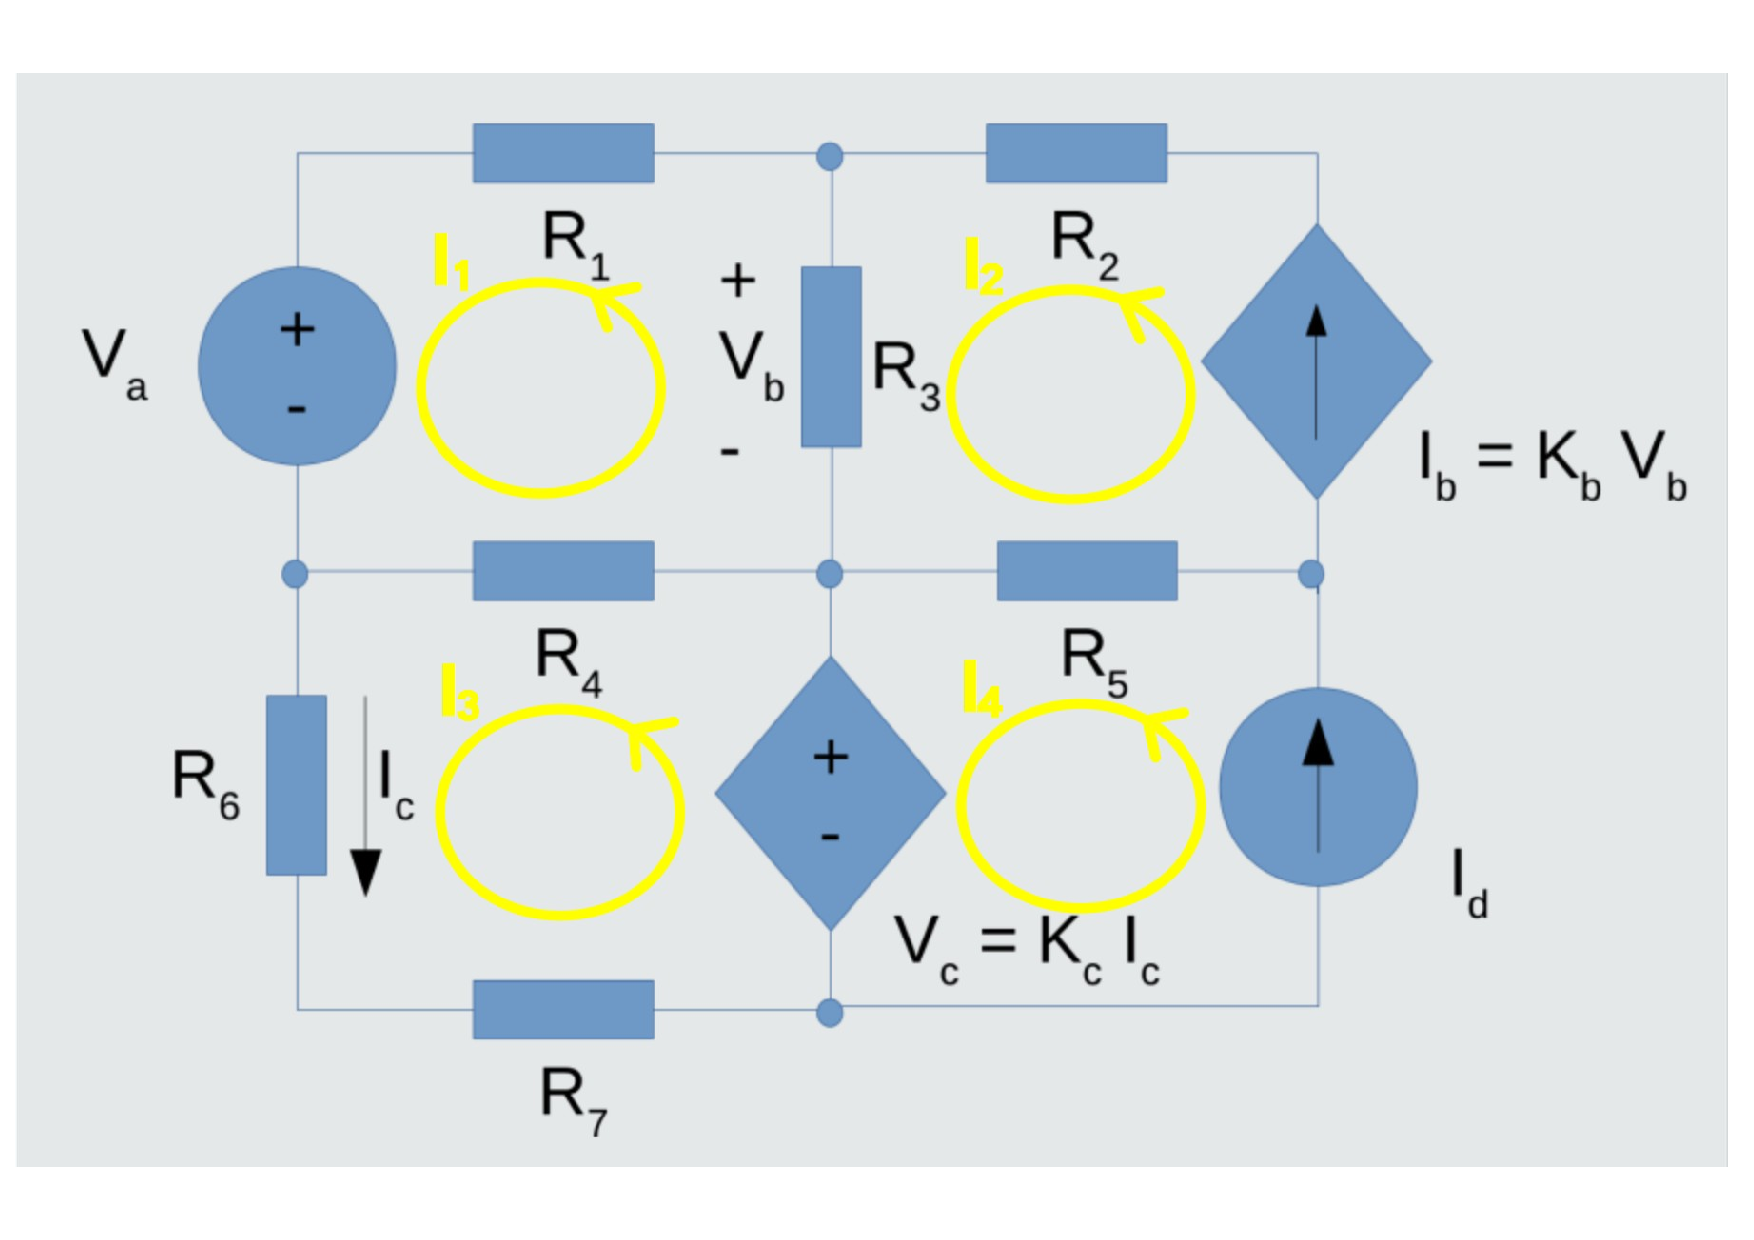
\includegraphics[width=0.7\linewidth]{meshcircuit.pdf}
\caption{Mesh currents}
\label{fig:mesh}
\end{figure}


The second step is to write Kirchhoff's Voltage Law equations around each mesh; however, the value of $I_d$ is already known, so there's no need to write an equation around the fourth mesh. This being said, and knowing by Ohm's Law that
\begin{equation}
  V=RI
\end{equation}

the equation for the first mesh is:

\begin{equation}
  V_a + R_4(I_1 - I_3) + R_3(I_1 - I_2) + R_1I_1 = 0 \Leftrightarrow I_1(R_1+R_3+R_4) - I_2R_3 - I_3R_4 = -V_a
  \label{eq:kvl}
\end{equation}

In the second mesh, noticing that $I_b=I_2$, $V_b$ can be written in two ways:

\[   V_b = \frac{I_2}{K_b}   \]
and
\[   V_b = R_3(I_2-I_1)   \]

Therefore:
\begin{equation}
\frac{I_2}{K_b} = R_3(I_2 - I_1)\Leftrightarrow I_2 = K_bR_3(I_2-I_1)\Leftrightarrow -I_1K_bR_3 + I_2(K_bR_3-1) = 0
  \label{eq:kvl}
\end{equation}

And finally, for the third mesh:
\begin{equation}
  R_6I_3 + R_7I_3 - V_c + R_4(I_3-I_1) = 0
  \label{eq:kvl}
\end{equation}

and since $V_c = K_cI_c$ and $I_c=I_3$:
\begin{equation}
 -I_1R_4 + I_3 (R_4+R_6+R_7-K_c) = 0
  \label{eq:kvl}
\end{equation}

The next step is to solve the resulting system of equations for the mesh currents:

\begin{equation}
\left(\begin{array}{ccc} R_1+R_3+R_4 & -R_3 & -R_4\\ -K_bR_3 & K_bR_3-1 & 0 \\ -R_4 & 0 & R_4+R_6+R_7-K_c \end{array}\right)
\left(\begin{array}{c} I_1 \\ I_2 \\ I_3 \end{array}\right) 
= \left(\begin{array}{c} -V_a \\ 0 \\ 0 \end{array}\right)
\end{equation}

